\section{Case Study: Rössler System}

The well known Rössler system is given by the equations
\[
	\begin{array}{rcl}
		\dot x &=& -y - z \\
		\dot y &=& x + a \cdot y \\
		\dot z &=& b + z \cdot (x - c) \\
	\end{array}
\]
with parameters $a$, $b$, and $c$. For this example, $a$ and $b$
are fixed to $0.1$, while we are varying $c$.

The system has several periodic solutions for each value of $c$ with different
periodicities, though only one is stable at a time. We are interested in the origin and
branching of those solutions and, thus, drawing a bifurcation diagram using the map
\[
	f \mapsto \{ \|f(t)\|_2  \ | \ t \in [0, 2\pi), \ f(t)_1 = 0 \} \ .
\]
Here, $f$ denotes a single periodic solution. Note, that we use only the approximation
given by Galerkin's method.

As a starting point, one might choose $c=4$. \dots

\begin{figure}[!ht]
	\centering
	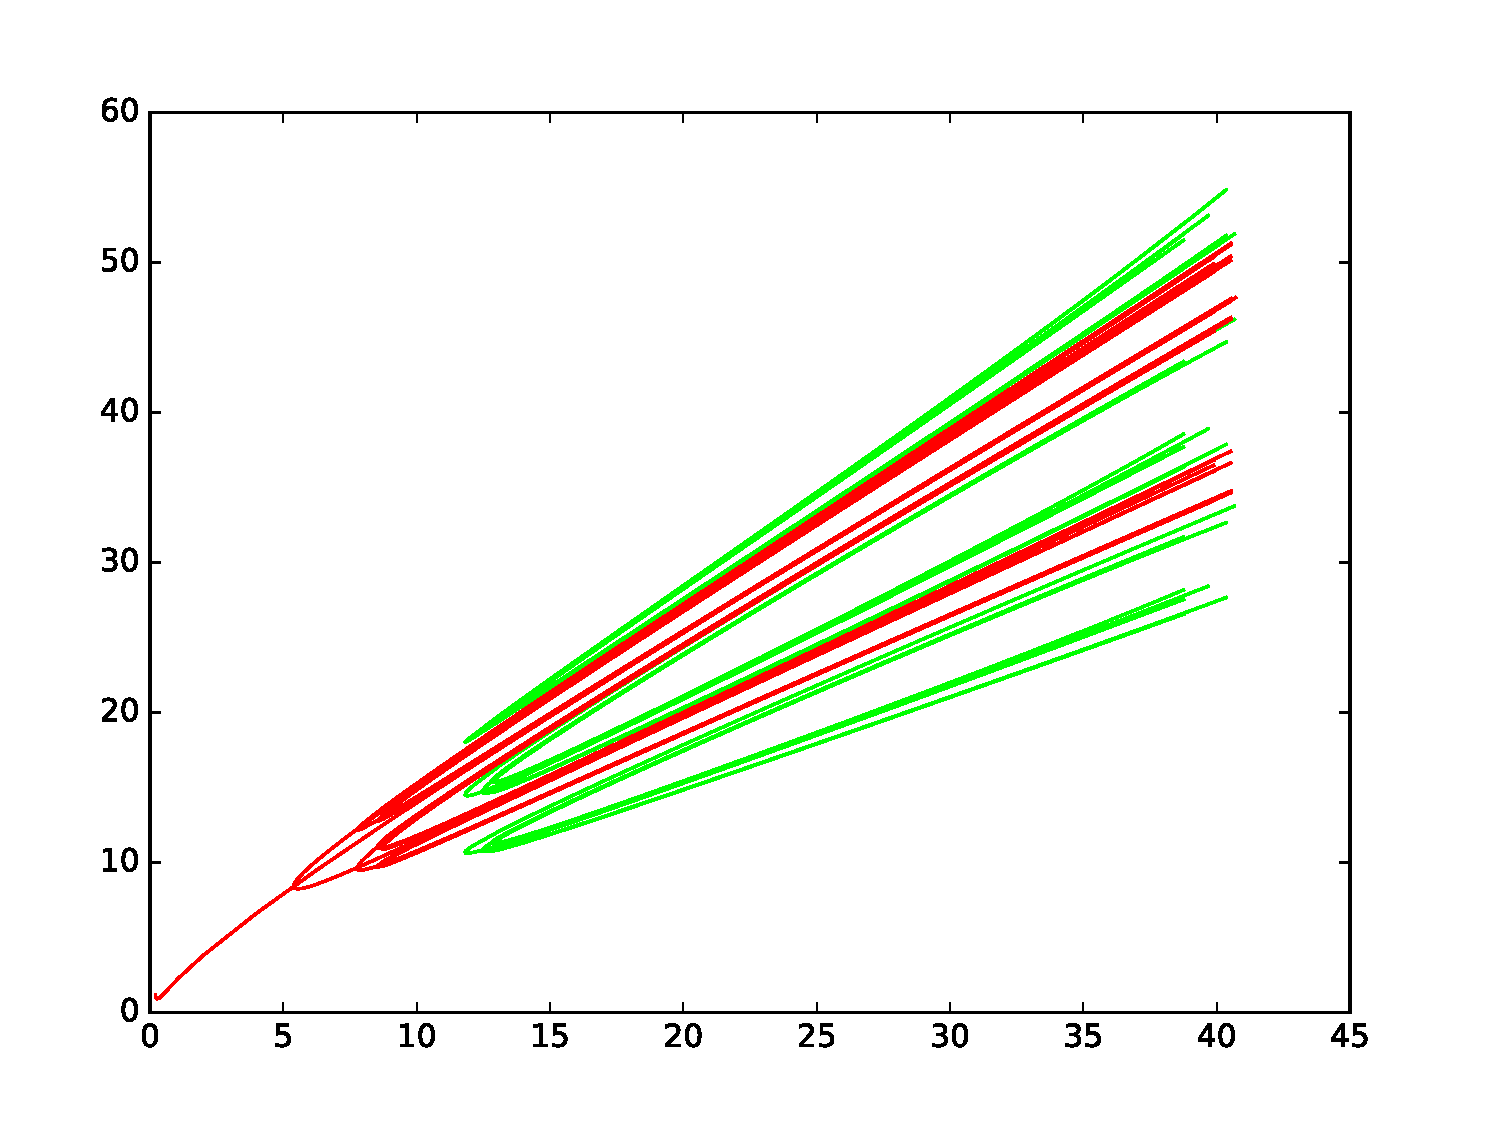
\includegraphics[width=1\textwidth]{img/roessler2a.pdf}
	\caption{The bifurcation diagram of the Rössler system for varying $c$. The
		even-periodic solutions are colored red, the odd-periodic ones green.}
\end{figure}

\begin{figure}[!ht]
	\centering
	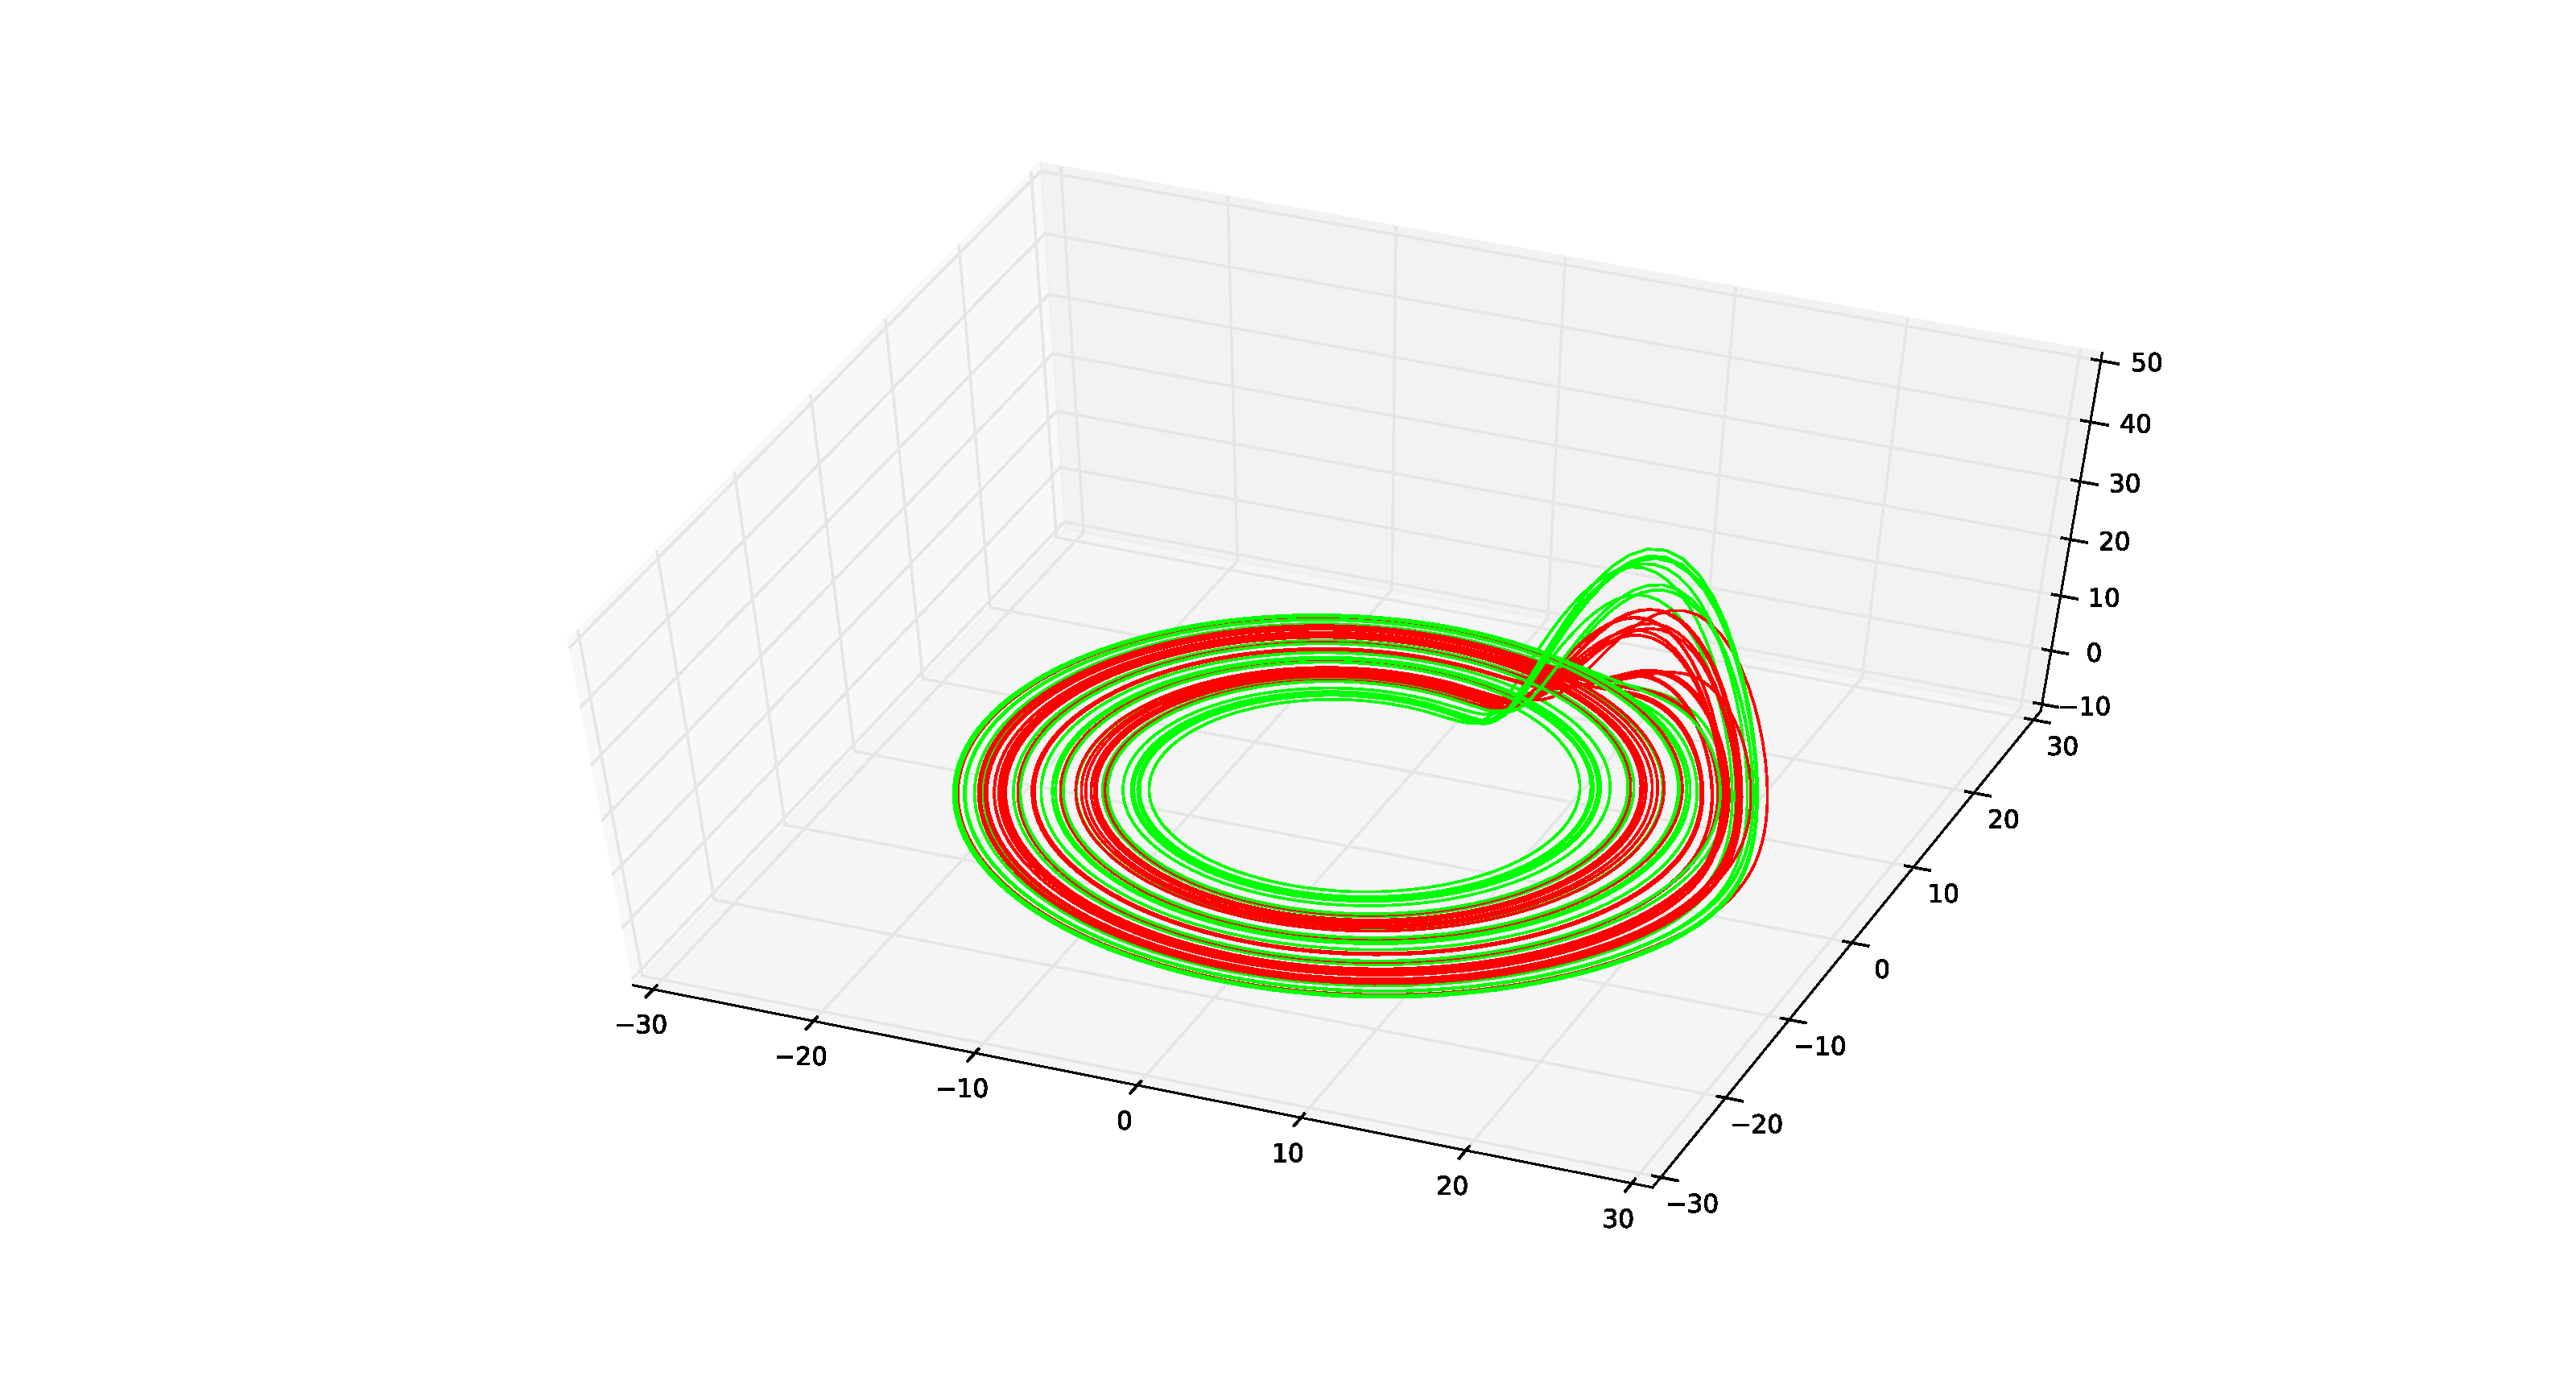
\includegraphics[width=1\textwidth]{img/roessler2b.pdf}
	\caption{All found solutions for $c=\dots$ plotted into one diagram.
	Observe how the odd-periodic and even-periodic solutions dodge since they do not
	originate from each other.}
\end{figure}



